\section{Security Model}
\label{sec:attestation}

The central context of SGX is the \textit{enclave}, a protected environment
that contains the code and data pertaining to a security-sensitive computation.

The rest of this section describes the security properties of
enclaves, discussing the trade-offs made while trying to balance security with
backwards compatibility.

Enclaves were designed to contain and protect the privacy-sensitive parts of an
application. All the code that handles private data must receive integrity
protection. Otherwise, a hostile environment could modify the code to leak
information about private data. Therefore, the SGX programming model prescribes
that code which accesses private data must be entirely contained inside an
enclave. Jumping into and out of enclave code must be performed explicitly
using the dedicated instructions \texttt{EENTER} and \texttt{EEXIT}.

The code inside an enclave runs at ring 3 (user mode), so it has the same
privileges as regular application code (see Figure \ref{fig:cpu_rings}).

\begin{figure}[hbtp]
  \center{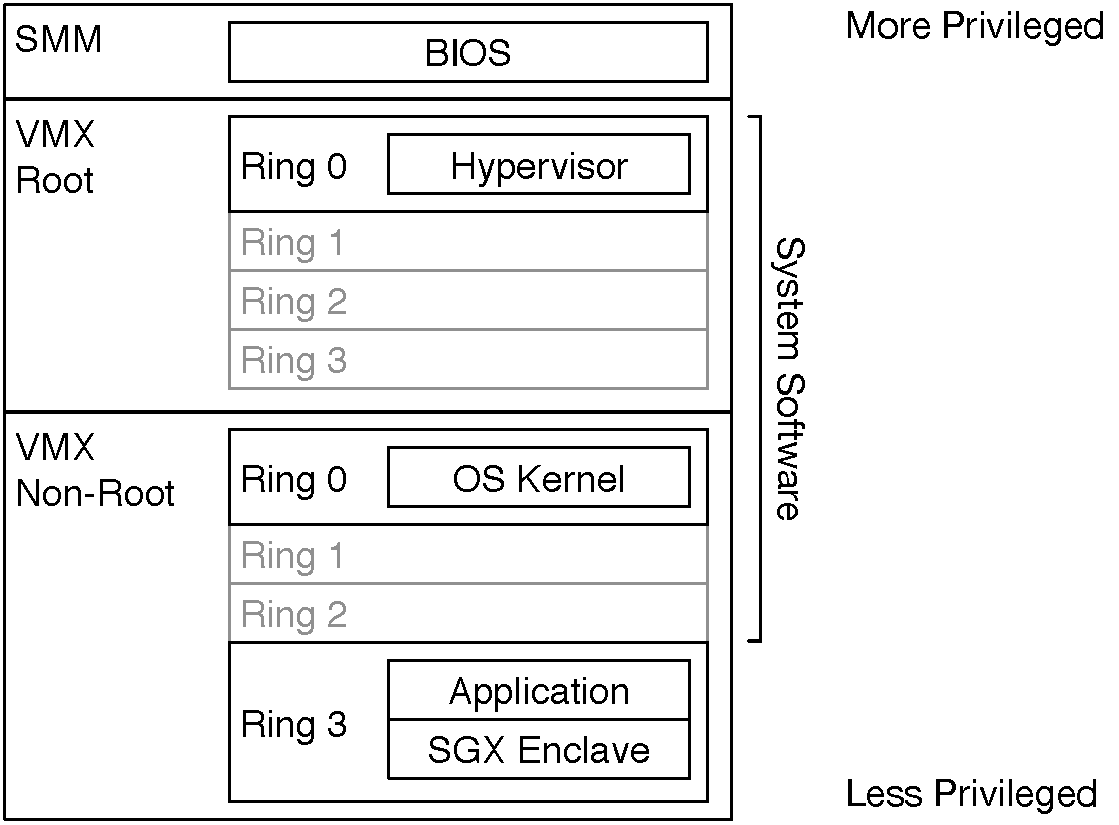
\includegraphics[width=75mm]{figures/cpu_rings.pdf}}
  \caption{
    Enclaves hold an application's private data and the code that operates on
    it. Therefore, they run at ring 3, in user mode.
  }
  \label{fig:computing_model}
\end{figure}
